\documentclass[10pt]{article}
\usepackage[T1]{fontenc}
\usepackage{lmodern,amsmath,amssymb,graphicx,hyperref}
\usepackage[margin=.74in]{geometry}
\setlength{\parindent}{0pt}\setlength{\parskip}{7pt}
\begin{document}
\begin{center}{\Large Explicit modular extraction and inverse}\\[4pt]
Local continuation --- 15 November 2026\end{center}
\textbf{Result.} The actual word entry now constructs its final quotient,
odd-unit inverse and multiplication using the proved word routines. Its value
agrees with the previous finite extraction and the canonical actual auxiliary
absoluteRight coefficient under the unchanged source premises. This closes
the final opaque modular arithmetic step at the component scope. Counts below
are emitted arithmetic XOR/AND/OR events, not all machine instructions or a
complete synthesized hardware circuit [pcc:unverified].

\textbf{Evidence.} Accepted060 has314 theorem statements, 061 has323, 062
has329, and063 has336, each including prior work and each with exit0 and no
warnings. Receipts032--035 bind exact sources, raw logs and exits. PCC suffixes
are respectively 04ea1d, e7f27f, f8275c and02762e, all prefixed
PCC-20261115-. Central printed dependencies are standard. This local evidence
is outside shared Transport53/57/fresh; all records remain unsigned and
not\_covered [pcc:unverified].

\textbf{Quotient before final reduction.} For the actual positive denominator
$d$, let $E=v_2(d)$ and $q=p+E$. The numerator is an actual width-$q$ word,
whose decoded integer is the canonical representative of its residue. Dropping
exactly $E$ low bits constructs a width-$p$ quotient word. The proof establishes
\[
 V_p(\operatorname{quotientWord}(w))
 =\left\lfloor\frac{\operatorname{val}(V_q(w))}{2^E}\right\rfloor
 \pmod {2^p}.
\]
The actual drop records its skipped bits and their length is exactly $E$.
The proof covers $E=0$, $p=0$ and canonical words produced from negative
source numerators. It does not divide by two inside the smaller ring or invert
two. List copying, control and storage still require accounting
[pcc:unverified].

\textbf{Derived odd unit.} Write $d=2^E b$ with $b=\operatorname{oddPart}(d)$.
Positivity comes from the actual denominator construction. Its oddness is
therefore derived, rather than supplied as a favorable unit witness.
For any commutative ring the constructed Newton recurrence satisfies
\[
 y_0=1,\quad y_{k+1}=y_k(2-by_k),\qquad
 1-by_k=(1-b)^{2^k}.
\]
The initial error is even, so in $\mathbb Z/2^p\mathbb Z$ the conservative
$p$-step schedule yields the canonical inverse of $b$. The proof retains
$p=0$; an even zero input in $\mathbb Z/2\mathbb Z$ is a control showing why
the oddness premise matters [pcc:unverified].

\textbf{Prior work.} Newton inversion and schoolbook word arithmetic are
standard. Brent and Zimmermann, \emph{Modern Computer Arithmetic}, author
PDF0.5.9, section2.5 equation2.3, supplies the squared-error recurrence;
section1.4.8 discusses fixed-word arithmetic. The pinned source review and
complete PDF digest are in literature-review-001.json. The book's fast
$O(M(n))$ bound is not inherited by this fixed-width implementation, and
fixed hardware wraparound is not free arbitrary-width preparation
[pcc:unverified].
\newpage
\begin{center}{\Large Constructed arithmetic events and actual driver}\end{center}
\textbf{Word inverse.} One actual step uses two word products, one negation
and one addition. The previous routines emit $5p^2$, $6p$ and $5p$ events,
respectively. Thus the actual step emits exactly $10p^2+11p$ events, and the
fixed-width $p$-step inverse emits exactly $10p^3+11p^2$. No runtime modular
inverse oracle appears in these new word helpers [pcc:unverified].

\textbf{Extraction composition.} A single actual drop feeds the quotient
word into the actual inverse and final word multiplication. The returned
canonical value equals finiteExtract. The extraction stage emits exactly
\[
 10p^3+16p^2
\]
arithmetic events and records exactly $E$ skipped bits. Constants, odd-part
construction, valuation, magnitude encoding and the branch/control operations
are not included in this arithmetic-event count [pcc:unverified].

\textbf{Actual auxiliary entry.} The completeEntry driver constructs the same
actual creation index, denominator and numerator as before. Let
\[
 \begin{aligned}
 k&=\operatorname{creationIndex}(p,\operatorname{jetWeight}),&
 q&=p+v_2(d),\\
 C(q,h,z)&=10(q+1)^2(hz+1)^2,& h&=b+1,\quad z=n+1.
 \end{aligned}
\]
Here $b$ is the label's degree index, distinct from the odd denominator above.
Using the previously proved actual syntax bound $N_*$, the complete driver's
emitted arithmetic-event count is bounded by
\[
 \boxed{C(q,b+1,n+1)N_*+6q+5q^2+10p^3+16p^2.}
\]
This follows from composed actual traces and the actual positive denominator,
without a unit oracle or a supplied operation-cost bound. The previous node,
valuation, crossing, label and port hypotheses are unchanged
[pcc:unverified].

\begin{center}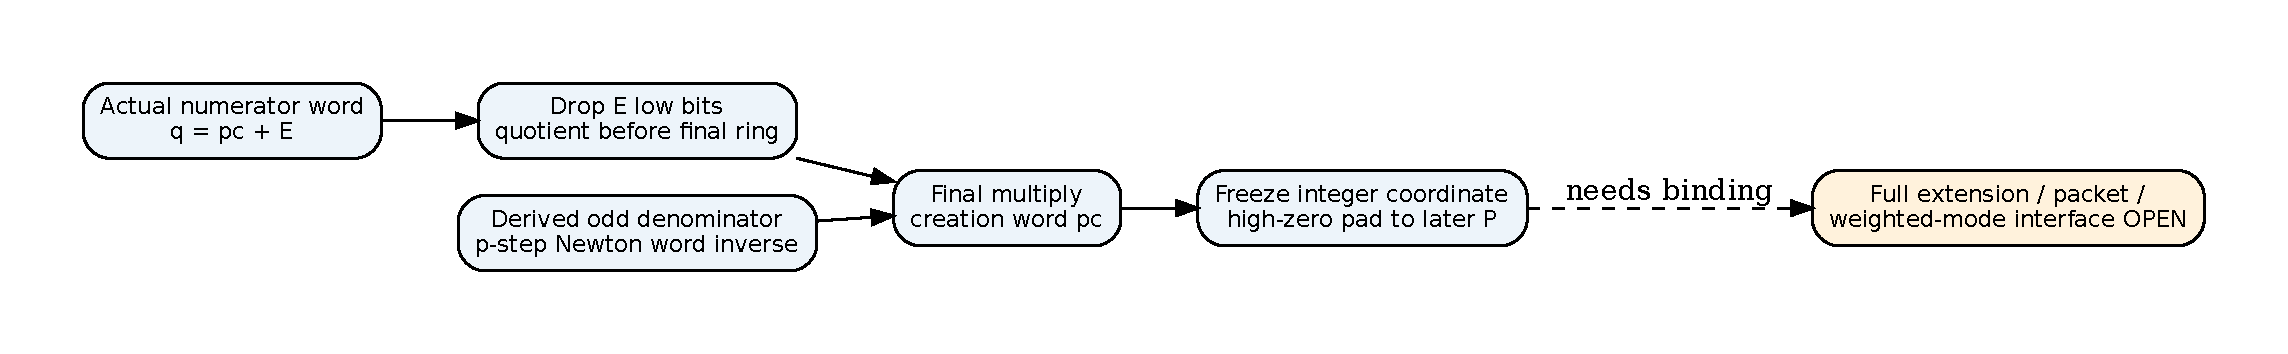
\includegraphics[width=\linewidth]{modular-completion-dependencies-001.pdf}\end{center}

\textbf{Costs still separate.} All scalar and rational preparation, actual
AST and denominator construction, integer magnitude encoding and halving,
constant preparation, selection and control, basis construction, array access,
index/bounds checks, trace concatenation, allocation and memory remain to be
charged. The old rational scalar preparation can still execute its own
arithmetic. Removing the final modular inverse oracle does not remove those
operations. Zero emitted events is not zero work, and instrumentation is not
assumed free to erase [pcc:unverified].

\textbf{Failures retained.} Failed059 precedes accepted060. Failed064 was an
administrative source-assembly path error, not a mathematical attempt;
failed065 and any successors are preserved with their raw outputs. Earlier
archives, claims, reports and failed sources remain exact. No native timing,
scaling or attack campaign was run [pcc:unverified].
\newpage
\begin{center}{\Large Immutable creation representatives}\end{center}
\textbf{Source contract.} The primary tensor text, D.4.1 and D.4.6, requires
an entry to be evaluated at its fixed creation precision $p_c$, then reuses
those same integer coordinate representatives at later precisions. It
explicitly disclaims a ring-homomorphism rule for this lifting. Native Ring
and Packet source already implement that contract: Packet evaluates at its
recorded creation precision, then lifts the coordinate residues. No defect
or new native experiment is claimed [pcc:unverified].

\textbf{Source receipt.} creation-contract-source-review-001.json pins exact
Git blobs for native Ring and contraction plus existing precision and cost
reviews. It also pins the preserved primary PDF at revision
7ef5c0cc5ca4 (full revision in the receipt), SHA256 beginning
5b1612dc2eeb. KB/theorem tools were unavailable; the review used the exact
primary and repository fallback. The source's claimed tensor theorem is not
independently certified by this compatibility review [pcc:unverified].

\textbf{Scalar adapter.} The new adapter stores the actual completeEntry
word at $p_c$ and appends $P-p_c$ high zero bits for $P\ge p_c$. Accepted067 (344 statements including prior336, exit0, no warnings) proves preservation of the decoded integer, equality with
casting that canonical integer into the later residue ring, successive-lift
coherence, and exact copied/padded payload lengths. It must bind to the
creation driver, rather than recompute its formula at $P$. Receipt036 binds this separately compiled adapter evidence; its eight new
statements are not inferred from the 336-statement modular compilation [pcc:unverified].

\textbf{Next interface.} The scalar adapter alone does not construct the
unramified extension and nilpotent-basis coordinate representation or the
original packet description. Those require a concrete adapter with the same
extension polynomial, immutable metadata and no callback composition hidden
inside new packets. The original entry bound depends on an explicit number
of affine factors and terms; it cannot be imported merely from canonical
scalar agreement [pcc:unverified].

\textbf{Discriminating mode obligation.} Before another recursive cost claim,
count the actual nonzero weighted modes of this family. Every $2^u k$ label
remains charged. Neither the earlier $2^{i+1}$ tile count nor declared capacity
proves the required density, nonzero inventory or independent rank. A reduction
needs actual coefficient valuations/support, valid matrix factors and the
child-entry/edge/degree interface. PROTOCOL-009.md records these next checks
[pcc:unverified].

\textbf{Evidence boundary.} This is the same auxiliary matrix family. The
original creation/packet/mode interface and full bit-runtime accounting remain
open, together with the actual elliptic relation, public finder, field/scalar
extraction, retries and complete expected cost. No additional origin channel
or elliptic relation map is supplied by modular arithmetic
[pcc:unverified].
\end{document}
